\documentclass[final]{beamer}

\usepackage[scale=1.24]{beamerposter} % Use the beamerposter package for laying out the poster

\usetheme{confposter} % Use the confposter theme supplied with this template

\setbeamercolor{block title}{fg=ngreen,bg=white} % Colors of the block titles
\setbeamercolor{block body}{fg=black,bg=white} % Colors of the body of blocks
\setbeamercolor{block alerted title}{fg=white,bg=dblue!70} % Colors of the highlighted block titles
\setbeamercolor{block alerted body}{fg=black,bg=dblue!10} % Colors of the body of highlighted blocks
% Many more colors are available for use in beamerthemeconfposter.sty

%-----------------------------------------------------------
% Define the column widths and overall poster size
% To set effective sepwid, onecolwid and twocolwid values, first choose how many columns you want and how much separation you want between columns
% In this template, the separation width chosen is 0.024 of the paper width and a 4-column layout
% onecolwid should therefore be (1-(# of columns+1)*sepwid)/# of columns e.g. (1-(4+1)*0.024)/4 = 0.22
% Set twocolwid to be (2*onecolwid)+sepwid = 0.464
% Set threecolwid to be (3*onecolwid)+2*sepwid = 0.708

\newlength{\sepwid}
\newlength{\onecolwid}
\newlength{\twocolwid}
\newlength{\threecolwid}
\setlength{\paperwidth}{48in} % A0 width: 46.8in
\setlength{\paperheight}{36in} % A0 height: 33.1in
\setlength{\sepwid}{0.024\paperwidth} % Separation width (white space) between columns
\setlength{\onecolwid}{0.22\paperwidth} % Width of one column
\setlength{\twocolwid}{0.464\paperwidth} % Width of two columns
\setlength{\threecolwid}{0.708\paperwidth} % Width of three columns
\setlength{\topmargin}{-0.5in} % Reduce the top margin size
%-----------------------------------------------------------

\usepackage{graphicx}  % Required for including images

\usepackage{booktabs} % Top and bottom rules for tables

\usepackage{natbib} % Top and bottom rules for tables

%----------------------------------------------------------------------------------------
%	TITLE SECTION
%----------------------------------------------------------------------------------------

\title{Bigger and Faster Stochastic Gradient Langevin Dynamics using MPI} % Poster title

\author{Feynman Liang} % Author(s)

\institute{CS 267, UC Berkeley} % Institution(s)

%----------------------------------------------------------------------------------------

\begin{document}

\addtobeamertemplate{block end}{}{\vspace*{2ex}} % White space under blocks
\addtobeamertemplate{block alerted end}{}{\vspace*{2ex}} % White space under highlighted (alert) blocks

\setlength{\belowcaptionskip}{2ex} % White space under figures
\setlength\belowdisplayshortskip{2ex} % White space under equations

\begin{frame}[t] % The whole poster is enclosed in one beamer frame

\begin{columns}[t] % The whole poster consists of three major columns, the second of which is split into two columns twice - the [t] option aligns each column's content to the top

\begin{column}{\sepwid}\end{column} % Empty spacer column

\begin{column}{\onecolwid} % The first column


%----------------------------------------------------------------------------------------
%	INTRODUCTION
%----------------------------------------------------------------------------------------

\begin{block}{Introduction}

  \begin{itemize}
    \item \textbf{Motivation}: Posterior samples $\theta_i \sim P(\theta \mid X)$ are useful
      for Bayesian statistics, e.g.\ Monte Carlo approximations
      $$n^{-1} \sum_{i=1}^n f(\theta_i) \to E_{P(\cdot \mid X)} f(\theta_i)$$
    \item \textbf{Goal}: Generate posterior samples in
      a data-parallel manner which makes efficient use of available compute resources
    \item \textbf{Challenges}:
      \begin{itemize}
        \item Typical MCMC require entire dataset
          to compute Metropolis-Hastings acceptance probability, limiting scalability
        \item Communication costs are non-trivial in distributed computing environments
        \item Worker speeds and data partitioning may be imbalanced, requiting non-trivial
          management to achieve good utilization
      \end{itemize}
  \end{itemize}

  % Bayesian statisticians oftentimes need to generate samples from a
  % posterior distribution $P(\theta \mid X)$.
  % Stochastic Gradient Langevin Dynamics (SGLD) \citep{welling2011bayesian} is
  % a recently proposed method for doing so whose key advantage over traditional MCMC
  % is that it only requires minibatches of data, enabling data-parallel scaling
  % to large datasets. Researchers \citep{ahn2014distributed}
  % have already exploited this data-parallelism to develop distributed SGLD (D-SGLD),
  % which used an AWS cloud environment where each compute instance is running on
  % commodity hardware and inter-process communication requires high-latency
  % network I/O. In this project, we build upon their work and research the
  % parallelization of SGLD within a high-performance computing cluster
  % environment.

  % Bayesian statisticians oftentimes need to estimate expectations over a
  % posterior distribution $P(\theta \mid X)$. An example of this is the
  % minimum mean square error estimator, which is defined as
  % $$\hat\theta(X) = E[\theta \mid X]$$
  % Unfortunately, explicit computation is oftentimes intractable,
  % motivating the use of Monte carlo approximations.
  % Given posterior samples $\theta_i \sim P(\cdot \mid X)$,
  % from which the law of large numbers and continuous mapping theorem ensure consistent estimation:
  % for any continuous function $f$, as $n \to \infty$
  % $$n^{-1} \sum_{i=1}^n f(\theta_i) \overset{a.s.}{\to} E_{P(\cdot \mid X)} f(\theta_i)$$

  % Stochastic Gradient Langevin Dynamics (SGLD) \citep{welling2011bayesian} is a
  % recently developed method for generating the required posterior samples $\theta_i$
  % which can be applied on small mini-batches. Researchers \citep{ahn2014distributed}
  % have already exploited this data-parallelism to develop distributed SGLD (D-SGLD).
  % However, D-SGLD was developed an AWS cloud environment where each compute
  % instance is running on commodity hardware and inter-process communication
  % requires high-latency network I/O. In this project, we build upon their work
  % and research the parallelization of SGLD within a high-performance computing
  % cluster environment.
\end{block}

\begin{block}{Our Method}
  \begin{itemize}
    \item Partition data into shards $(X_s)_{s \in S}$
    \item Using MPI, perform distributed stochastic gradient Langevin dynamics (D-SGLD) \cite{ahn2014distributed}
      \begin{align}
        \Delta \theta = \frac{\epsilon_t}{2}\left( \nabla \log P(\theta) + N g(\theta_t, X_s) \right) + \nu_t
      \end{align}
      where $\nu_t \overset{\text{iid}}{\sim} N(0, \epsilon_t)$, $\epsilon_t \to 0$ sufficiently slowly,
      $g(\theta_t, X_s)$ unbiased estimator of $\nabla \log P(\theta \mid X_s)$.
  \end{itemize}

  In addition, we explored the following optimziations and modifications
  \begin{itemize}
    \item Trajectory sampling to avoid short communication cycles and
      trade off between communication overhead and mixing rates \citep{ahn2014distributed}
    \item Trajectory length load balancing to improve utilization \citep{ahn2014distributed}
    \item Stochastic gradient Riemannian Langevin dyanmics (SGRLD) to sample
      parameters constrainted to the probability simplex \cite{patterson2013stochastic}
  \end{itemize}


\end{block}

%%------------------------------------------------

%\begin{figure}
%
\includegraphics[width=0.8\linewidth]{placeholder.jpg}
%\caption{Figure caption}
%\end{figure}

%%----------------------------------------------------------------------------------------

\end{column} % End of the first column

\begin{column}{\sepwid}\end{column} % Empty spacer column

\begin{column}{\twocolwid} % Begin a column which is two columns wide (column 2)

\begin{columns}[t,totalwidth=\twocolwid] % Split up the two columns wide column

\begin{column}{\onecolwid}\vspace{-.6in} % The first column within column 2 (column 2.1)

%----------------------------------------------------------------------------------------
%	MATERIALS
%----------------------------------------------------------------------------------------

\begin{block}{Parallel chains and chain exchange}
  Experiments consider a Gaussian mixture model (GMM) with
  priors $\theta_1 \sim \mathcal{N}(0,10)$, $\theta_2 \sim \mathcal{N}(0,1)$
  and likelihood
  $x_i \overset{\text{iid}}{\sim} \frac{1}{2}\mathcal{N}(\theta_1, 2) + \frac{1}{2}\mathcal{N}(\theta_1 + \theta_2, 2)$.
  This model has a mode at $\theta_1 = 0$, $\theta_2 = 1$ as well as at
  $\theta_1 = -1$, $\theta_2 = 1$ and exhibits negative correlation
  between the parameters.

  \begin{figure}
    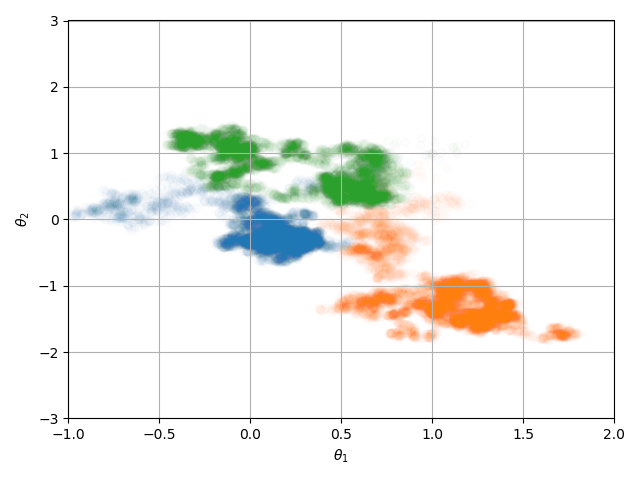
\includegraphics[width=0.8\linewidth]{poster-figures/gaussian_no_exchange.png}\\
    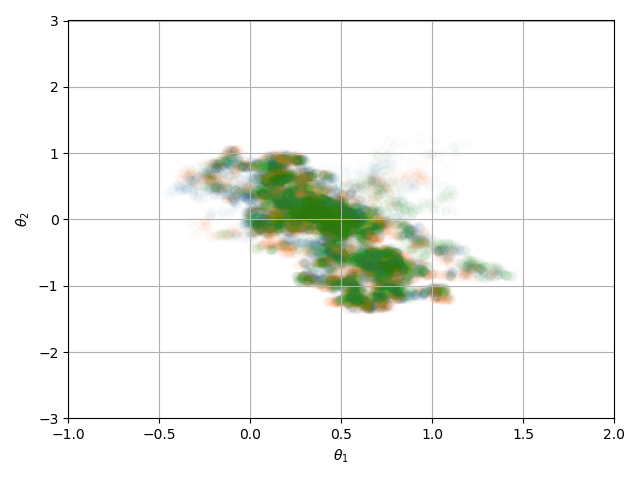
\includegraphics[width=0.8\linewidth]{poster-figures/gaussian_exchange.png}
    \caption{Samples drawn from local posteriors $P(\theta \mid X_s)$ (top, e.g.\ due to lack
      of chain exchange) may not well approximate the global posterior
      $P(\theta \mid \cup_s X_s)$ (bottom).}
    \label{fig:samples}
  \end{figure}
  \vspace{-2cm}
  \begin{figure}
    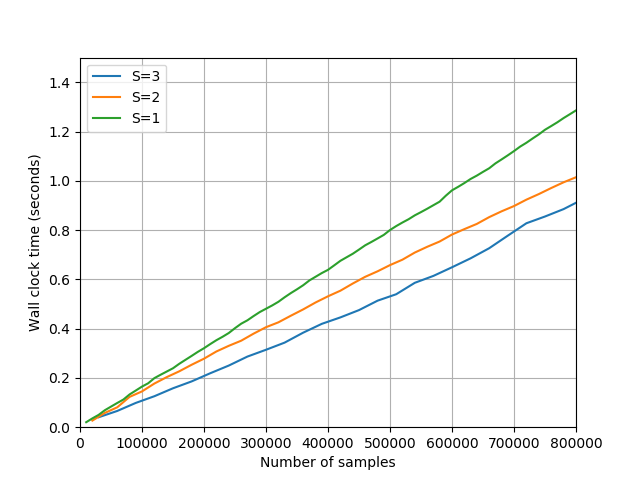
\includegraphics[width=0.9\linewidth]{poster-figures/speedup-parallel.png}
    \caption{Speedups due to parallelism.}
    \label{fig:speedup-partitioning}
  \end{figure}

\end{block}

%----------------------------------------------------------------------------------------

\end{column} % End of column 2.1

\begin{column}{\onecolwid}\vspace{-.6in} % The second column within column 2 (column 2.2)

%----------------------------------------------------------------------------------------
%	METHODS
%----------------------------------------------------------------------------------------

\begin{block}{Trajectory sampling}
  % Exchanging chains after each iteration incurs significant communication overhead.
  % To circumvent this, SGLD can be modified to perform trajectory sampling.
  % Instead of drawing a single sample, a trajectory of length $\tau$ is sampled
  % on each worker prior to exhanging chains. This can reduce the amount of inter-worker
  % communication (Figure~\ref{fig:less-comm}), but it must be used with care as too little
  % chain exchange results in biased samples as seen in Figure~\ref{fig:travelling-chain-samples}.
  \begin{figure}
    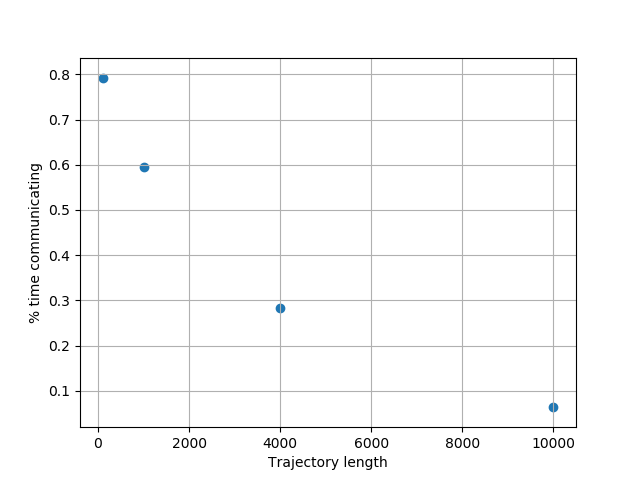
\includegraphics[width=0.7\linewidth]{poster-figures/traj_length_slowdown.png}
    \caption{Increasing trajectory length reduces how often communication happens, resulting in less
      communication overhead.}
    \label{fig:less-comm}
  \end{figure}
\end{block}
\vspace{-2cm}

\begin{block}{Trajectory length load balancing}

  \begin{figure}[htpb]
    \centering
    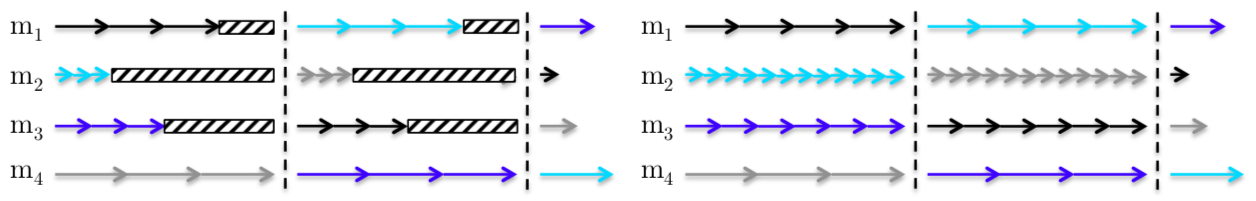
\includegraphics[width=1.0\linewidth]{poster-figures/ahn-lb.png}
    \caption{Figure from \cite{ahn2014distributed} showing the changes in worker
      utilization before and after load balancing.}
    \label{fig:ahn-lb}
  \end{figure}

  \begin{figure}
    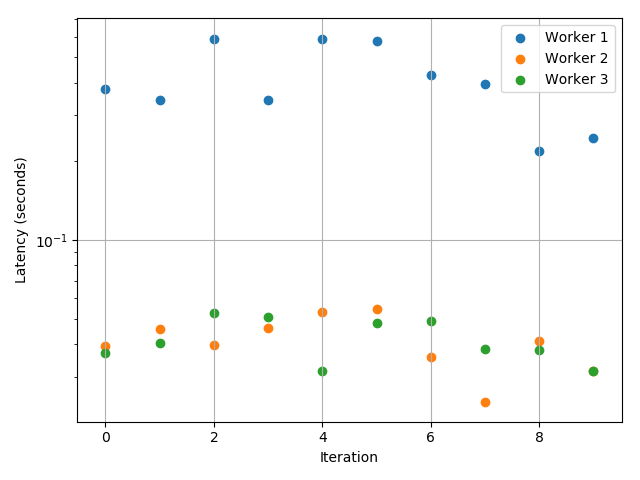
\includegraphics[width=0.7\linewidth]{poster-figures/load-balancing-none.png}\\
    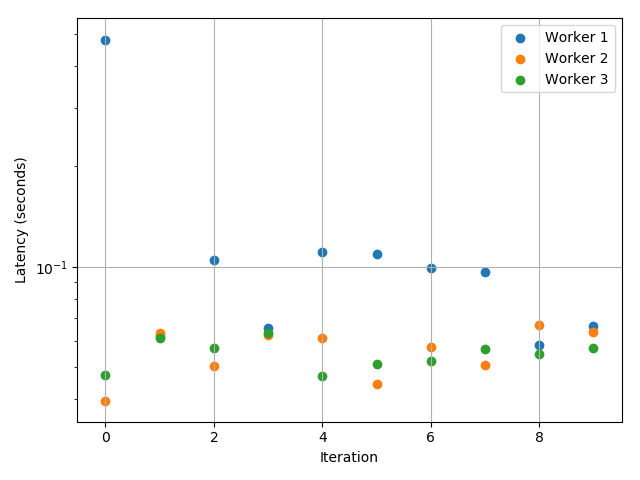
\includegraphics[width=0.7\linewidth]{poster-figures/load-balancing.png}
    \caption{Before (top) and after (bottom) trajectory length load balancing. Experiments used
      the previous GMM with an imbalanced data partioning which assigned 95\% to worker 1.}
    \label{fig:load-balancing}
  \end{figure}

%   Even with trajectory sampling, exchanging chains at the end of each trajectory necessitates
%   a mandatory global barrier synchronization. This results in a ``block on the slowest'' issue where
%   the fast workers sit idle waiting for the slower workers to complete (Figure~\ref{fig:load-balancing} left).
%   To improve utilization, worker-specific trajectory lengths $(\tau_s)_{s \in S}$ can be used to balance work
%   so that faster workers can continue to generate samples while waiting.

\end{block}


%----------------------------------------------------------------------------------------

\end{column} % End of column 2.2

\end{columns} % End of the split of column 2 - any content after this will now take up 2 columns width


\end{column} % End of the second column

\begin{column}{\sepwid}\end{column} % Empty spacer column

\begin{column}{\onecolwid} % The third column

\begin{block}{Latent Dirichlet Allocation}
  \begin{figure}
    \centering
    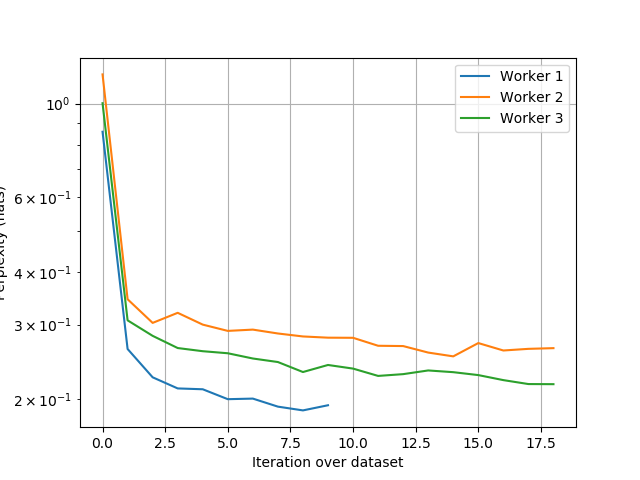
\includegraphics[width=0.8\linewidth]{poster-figures/perplexity-sgrld.png}
    \caption{Distributed SGRLD \cite{patterson2013stochastic} training of a LDA topic model.}
    \label{fig:perplexity-sgrld}
  \end{figure}
\end{block}

%----------------------------------------------------------------------------------------
%	CONCLUSION
%----------------------------------------------------------------------------------------

\begin{block}{Conclusion}

  We provide a novel implementation of D-SGLD on top of MPI and investigate the performance
  characteristics of various optimizations. Our results demonstrate that D-SGLD enjoys
  significant speedups due to parallelism, can sample posteriors even when data is partitioned
  disjointly across workers, and can be controlled using trajectory lengths to trade off
  between communication versus mixing time as well as load balance workers.
\end{block}

%----------------------------------------------------------------------------------------
%	ADDITIONAL INFORMATION
%----------------------------------------------------------------------------------------

% \begin{block}{Additional Information}

% Maecenas ultricies feugiat velit non mattis. Fusce tempus arcu id ligula varius dictum.
% \begin{itemize}
% \item Curabitur pellentesque dignissim
% \item Eu facilisis est tempus quis
% \item Duis porta consequat lorem
% \end{itemize}

% \end{block}

%----------------------------------------------------------------------------------------
%	REFERENCES
%----------------------------------------------------------------------------------------

\begin{block}{References}

\nocite{*} % Insert publications even if they are not cited in the poster
\small{\bibliographystyle{unsrt}
\bibliography{sample}\vspace{0.75in}}

\end{block}

%----------------------------------------------------------------------------------------
%	ACKNOWLEDGEMENTS
%----------------------------------------------------------------------------------------

% \setbeamercolor{block title}{fg=red,bg=white} % Change the block title color

% \begin{block}{Acknowledgements}

% \small{\rmfamily{Nam mollis tristique neque eu luctus. Suspendisse rutrum congue nisi sed convallis. Aenean id neque dolor. Pellentesque habitant morbi tristique senectus et netus et malesuada fames ac turpis egestas.}} \\

% \end{block}

%----------------------------------------------------------------------------------------
%	CONTACT INFORMATION
%----------------------------------------------------------------------------------------

\setbeamercolor{block alerted title}{fg=black,bg=norange} % Change the alert block title colors
\setbeamercolor{block alerted body}{fg=black,bg=white} % Change the alert block body colors

% \begin{alertblock}{Contact Information}

% \begin{itemize}
% \item Web: \href{http://www.university.edu/smithlab}{http://www.university.edu/smithlab}
% \item Email: \href{mailto:feynman@berkeley.edu}{john@smith.com}
% \item Phone: +1 (000) 111 1111
% \end{itemize}

% \end{alertblock}

% \begin{center}
% \begin{tabular}{ccc}
% 
\includegraphics[width=0.4\linewidth]{logo.png} & \hfill & 
\includegraphics[width=0.4\linewidth]{logo.png}
% \end{tabular}
% \end{center}

%----------------------------------------------------------------------------------------

\end{column} % End of the third column

\end{columns} % End of all the columns in the poster

\end{frame} % End of the enclosing frame

\end{document}
